\documentclass[../algebraNotesMSRI-UP2016.tex]{subfiles}

\begin{document}

\section[\S \thesection]{Diagonalization of integer matrices}\label{sec:2p9diagonalizationOfIntegerMatrices}
% % % % %
\subsection[\subsecname]{Linear algebra}\label{subsec:linearAlgebra}
% % %
\begin{frame}{\subsecname}
\begin{dfn}
Any group isomorphic to $\Z^n$, for some $n\in\N$, is called a \vocab{free abelian group of rank $n$}.
\end{dfn}

\smallGap
\begin{ex}
The subgroups $2\Z$, $3\Z$, $12\Z$, etc. in $\Z$ are all free of rank $1$.
\end{ex}

\smallGap
The group $\Z^n$ is analogous to the vector space $\R^n$; for example, the definitions of rank coincide.  In this spirit, we shall call $n$-tuples in $\Z^n$ \vocab{vectors}.
\end{frame}

% % %
\begin{frame}{}{}
\begin{dfn}%\label{dfn:independent}
Let $G$ denote a finitely generated abelian group and suppose $S=\{\vect g_1,\dots,\vect g_k\}\subset G$.
\begin{enumerate}[(a)]
\item $S$ is \vocab{independent} means if  
\begin{equation}\label{eq:independence}
a_1\vect g_1+\cdots+a_k\vect g_k=0\text{ with $a_i\in \Z$ for all $i=1,\dots,k$},
\end{equation}
then $a_i=0$ for all $i=1,\dots, k$.  
\item Any instance where Equation \eqref{eq:independence} fails is called a \vocab{relation}.
\item $S$ is a \vocab{basis} means it is independent and generates $G$.
\end{enumerate}
\end{dfn}

\smallGap
The vectors $\vect e_i$ defined in Section \ref{subsec:FGAG} are called \vocab{standard basis vectors}.  
\end{frame}

% % %
\begin{frame}
\begin{exe}\label{exe:uniqueSum}
Let $G\cong \Z^n$.  Use Equation \eqref{eq:independence} to show that if $S\subset G$ forms a basis for $G$ then every vector $\vect g\in G$ has a unique expression as a ($\Z$)-linear combination of the elements in $S$.
\end{exe}

\smallGap
A finitely generated abelian group has a basis if and only if it is free.  Free abelian groups are also called \vocab{torsion-free}, where \vocab{torsion} arises precisely from relations on generators.  In a group with torsion, there exist non-identity elements with finite order.  

\smallGap
\textbf{Caution:} Torsion-free does not imply free!  For example, the group $\Z\times \Z/2\Z$ is torsion-free but not free. 

\smallGap
Using bases, we have a concise way to express homomorphisms between (finitely generated) free abelian groups. 
\end{frame}

% % %
\begin{frame}
Suppose $\{\vect b_1,\dots,\vect b_n\}$ is a basis for $G\cong \Z^n$ and $\{\vect c_1,\dots,\vect c_m\}$ is a basis for $H\cong \Z^m$.  Let $\varphi:G\to H$ denote a group homomorphism such that  
\[
\varphi{(\vect b_j)}=\sum_{i=1}^ma_{ij}\vect c_i,\quad j=1,\dots,n
\]
for integers $a_{ij}$.  Let $A$ denote the $m\times n$ integer matrix whose $(i,j)$th entry is $a_{ij}$ for $i=1,\dots,m$ and $j=1\dots, n$.

\smallGap
By Exercise \ref{exe:uniqueSum}, every element in $G$ can be written $\vect g=g_1\vect b_1+\cdots g_n\vect b_n$ for unique $g_1,\dots, g_n\in \Z$.  

\vspace{-0.5pc}
Let us abuse notation and write 
$\vect g=(g_1,\dots,g_n)
	=\begin{pmatrix}
	g_1 \\
	\vdots \\
	g_n
	\end{pmatrix}
$.
\end{frame}

% % %
\begin{frame}{}{}
In this way we can write
\begin{multline*}
\varphi:\vect g \mapsto 
	\begin{pmatrix}
		a_{11} & a_{12} & \cdots & a_{1n} \\
		a_{21} & a_{22} & \cdots & a_{2n} \\
		\vdots & \cdots & \ddots & \vdots \\
		a_{m1} & a_{m2} & \cdots & a_{mn}
		\end{pmatrix}
	\begin{pmatrix}
		g_1 \\
		g_2 \\
		\vdots \\
		g_n\end{pmatrix}
	\\	
	= \begin{pmatrix}
		a_{11}g_1+a_{12}g_2+\cdots +a_{1n}g_n \\
		a_{21}g_1+a_{22}g_2+\cdots +a_{2n}g_n \\
		\vdots \\
		a_{m1}g_1+a_{m2}g_2+\cdots +a_{mn}g_n 
		\end{pmatrix} 
	= A\vect g.
\end{multline*}
In other words, the homomorphism $\varphi$ is left multiplication by $A$.  
\end{frame}

\begin{frame}[c]{}{}
\textbf{Summary:} Upon choosing bases for $G\cong \Z^n$ and $H\cong \Z^m$, we can express $\varphi:G\to H$ using the matrix $A$.  We simply define $\varphi$ by assigning an image to each of the basis elements of $G$... the caveat, of course, is the dependence on choice of bases.

\smallGap
\begin{que}
How do we get around this caveat?
\end{que}
\end{frame}

% % % % %
\subsection[\subsecname]{Normalizing}\label{subsec:normalizing}
% % %
\begin{frame}{\subsecname}
\textbf{Recall:} In Linear Algebra, given bases $\mathfrak B=\{\vect b_1,\dots,\vect b_n\}\subset \R^n$ and $\mathfrak C=\{\vect c_1,\dots,\vect c_n\}\subset \R^n$ we have a \vocab{change of basis matrix} obtained by writing the vectors $\vect b_j\ (j=1,\dots,n)$ as linear combinations of the vectors $\vect c_i\ (i=1,\dots,n)$.  The matrix is $U=(u_{ij})$, where
\[
\vect b_j=\sum_{i=1}^nu_{ij}\vect c_i,\quad j=1,\dots,n.
\]
Note, $U$ is necessarily invertible.  Left multiplication by $U$ expresses vectors with respect to $\mathfrak B$ as vectors with respect to $\mathfrak C$; given $\vect v=\sum_{j=1}^nv_j\vect b_j$ put $\vect w:=U\vect v$.  Then $U\1\vect w=\vect v$.
\end{frame}

% % %
\begin{frame}
\begin{ex}
Suppose $\R^n$ has basis $\mathfrak B=\{\vect b_1,\dots,\vect b_n\}$ and $\varphi:\R^n\to \R^n$ is a linear transformation given, with respect to $\mathfrak B$, by the matrix $B$.  For $\vect v=\sum_{j=1}^nv_j\vect b_j$, define
\[
\varphi_{\mathfrak B}:\vect v \mapsto B\vect v.
\]
Suppose $\mathfrak C=\{\vect c_1,\dots,\vect c_n\}$ is also a basis for $\R^n$ and we have a change of basis matrix from $\mathfrak B$ to $\mathfrak C$ given by $U=(u_{ij})$.  Because a change of basis is an isomorphism from $\R^n$ to $\R^n$ (also called an \vocab{automorhpism} on $\R^n$), for $\vect w=\sum_{i=1}^nw_i\vect c_i\in \R^n$, we may write $\vect v=U\1\vect w$ for some $\vect v\in \R^n$.  Then    
\[
\varphi_{\mathfrak C}:\vect w\mapsto UB\vect v=UBU\1\vect w
\]
gives the same transformation $\varphi$, but with respect to $\mathfrak C$.
\end{ex}
\end{frame}

% % %
\begin{frame}[c]
The conjugation of $B$ by $U$ is equivalent to performing row and column operations on $B$.  Left multiplication by $U$ performs the row operations and right multiplication by $U\1$ performs the column operations.  Furthermore, there is always a %unique 
basis $\mathfrak E$ such that $\varphi_{\mathfrak E}$ is given by (left) multiplication by a \vocab{normalized} matrix $E$, a matrix consisting of zeros everywhere except for 1s on the first $r\leq n$ diagonal entries.  Furthermore, we attain $E$ by row and column reducing $B$.

\smallGap
We call the process of attaining the basis $\mathfrak E$ \vocab{normalizing} the matrix $B$.
\end{frame}

% % %
\begin{frame}
More generally, a linear transformation $\R^n\to \R^m$ given by a matrix $A$ can be expressed as left multiplication by a normalized matrix $D=BAC$, where $B$ is an $n\times n$ invertible matrix which applies row operations to $A$, and $C$ is an $m\times m$ matrix performing column operations on $A$.

\smallGap
For the most part, we can apply these same ideas to integer matrices.  But keep in mind $\Z^n$ does not quite have the structure of $\R^n$.  One of the permissible matrix operations in $\Mat_{\R}(m,n)$ is scalar multiplication.  A scalar is just a non-zero number in $\R$.  But what characterizes a scalar is its existence of an inverse.  In $\Z$ the only scalars, or \vocab{units}, are $\pm 1$.  Hence when we perform matrix operations we are only allowed to divide by $\pm 1$.

\smallGap
\begin{que}
How does the normalization process change for integer matrices?  
\end{que}
\end{frame}

% % %
\begin{frame}
Suppose $\varphi: G\to H$ is a group homomorphism where $G\cong \Z^n$ and $H\cong \Z^m$.  It would be very convenient to find bases $\mathfrak B=\{\vect b_1,\dots,\vect b_n\}\subset G$ and $\mathfrak C=\{\vect c_1,\dots,\vect c_m\}\subset H$ so that for some $r\leq n,m$,
\[
\varphi(\vect b_i)
	=\begin{cases}
		\vect c_i & i\leq r \\
		0 & i>r
	\end{cases}.
\]
Suppose $\varphi$ is given by the $m\times n$ integer matrix $A$.  Since $\Z\subset\R$, the following operations are permissible:
\begin{itemize}
\item add an integer multiple of one column (resp. row) to another
\item interchange two columns (resp. rows)
\item multiply a column (resp. row) by $\pm 1$
\end{itemize}  
\end{frame}

% % %
\begin{frame}[c]
Under these constraints, the desired matrix $D$ will not be normalized, per se, but it will be diagonal.  Theorem \ref{thm:SmithNormalForm} gives an algorithm for producing a \vocab{canonical}, or standardized,
$m\times n$ diagonal matrix $D$, given an $m\times n$ integer matrix $A$.  The algorithm in Theorem \ref{thm:SmithNormalForm} produces a unique such matrix $D$.  
\end{frame}

% % % % %
\subsection[\subsecname]{Smith normal form}
% % %
\begin{frame}{\subsecname}
\begin{thm}[Smith normal form]\label{thm:SmithNormalForm}
Let $A$ denote an $m\times n$ integer matrix.  There exists an invertible $n\times n$ matrix $B$ and an invertible $m\times m$ matrix $C$ such that 

\[
D:=BAC=\begin{pmatrix}
	d_1 & 0 & \cdots & & & 0 \\
	0 & \ddots & \ddots & & & \vdots \\
	\vdots & \ddots & d_r & & & \\
	 & & & 0 & & & \\
	 & & & & \ddots &  \\
	0 & \cdots & & & & 0 \\	
	\end{pmatrix}
\]

for some $r\leq n,m$ and $d_i|d_{i+1}$ for each $i=1,\dots,r-1$.  In other words, each successive diagonal entry is an integer multiple of the last. 
\end{thm}  
\end{frame}

% % %
\begin{frame}{}{}
$D$ is called the \vocab{Smith normal form} of $A$.

\bigProof
We shall perform a sequence a row and column operations which culminate the invertible matrices $B,C$.  At each step we let $A=(a_{ij})$ denote the resulting matrix.  Let $R_i$ denote the $i$th row of $A$ and let $C_j$ denote the $j$th column.    

\smallGap
\textbf{Step 1:} Locate the entry $a$ with the smallest non-zero absolute value and permute rows and columns until $a_{11}=a$.  If $a<0$ then replace $R_1$ with $-R_1$.  

\smallGap
\textbf{Step 2:} Clear the first column; given a a non-zero entry $a_{i1}$, write 
\[
a_{i1}= aq+r,
\]  
where $q,r$ are as in the Division Algorithm (Equation \eqref{eq:divisionAlgorithm}).  In particular, $r<a$.  Replace $R_i$ with $R_i-qR_1$, and if $r\neq 0$, return to Step 1.  
\end{frame}

% % %
\begin{frame}
Repeating this process, each time we return to Step 1 the entry $a$ gets strictly smaller.  It will only take finitely many repetitions before either $a_{i1}=0$ for all $i$ or $a=1$.  But if $a=1$ then Step 2 is required at most more time per entry to clear any remaining non-zero entries in the $1$st column.  

\smallGap
Clear the first row using an analogous process; given a non-zero entry $a_{1j}$, write
\[
a_{1j}=aq+r
\]
as in the Division Algorithm and replace $C_j$ with $C_j-qC_1$.  If $r\neq 0$ then return to Step 1.  After finitely many repetitions $a$ will be the only non-zero entry in the first row.

\smallGap
\textbf{Step 3:} Ensure the divisibilty condition; let $B$ denote the submatrix of $A$ given by omitting its first row and column.  If an entry $b$ of $B$, in the $j$th column of $A$, does not divide $a$, then replace $C_1$ with $C_1+C_j$.  The first column of $A$ is no longer cleared so return to Step 2.
\end{frame}

% % %
\begin{frame}[c]
In Step 2 the Divison Algorithm will either replace $b$ with zero or else direct us back to Step 1 where the entry $a$ will become strictly smaller.  Hence this process will end after finitely many steps.
\qed

\smallGap
The divisibility condition on the diagonal entries simply gives a canonical form for the matrix $D$ and ensures its uniqueness.

\smallGap 
The algorithm in the proof of Theorem \ref{thm:SmithNormalForm} is more clear when seen in an example.
\end{frame}

% % %
\begin{frame}{}{}
\begin{ex}\label{ex:diagonalAlgorithm}
Here, we apply the algorithm from Theorem \ref{thm:SmithNormalForm} to a matrix $A$.
\begin{multline*}
A:=\begin{pmatrix*}[r]
	1 & -1 & 1 \\
	5 & 1 & -5 \\
	-3 & -3 & 29 
	\end{pmatrix*}\xrightarrow{\substack{C_2\to C_2+C_1 \\ C_3\to C_3-C1}}
\begin{pmatrix*}[r]
1 & 0 & 0 \\
5 & 6 & -10 \\
-3 & -6 & 32 
\end{pmatrix*} \\
\xrightarrow{\substack{R_2\to R_2-5R_1 \\ R_3\to R_3+3R_1}}
\begin{pmatrix*}[r]
1 & 0 & 0 \\
0 & 6 & -10 \\
0 & -6 & 32
\end{pmatrix*}\xrightarrow{C_3\to C_3+2C_2}
\begin{pmatrix*}[r]
1 & 0 & 0 \\
0 & 6 & 2 \\
0 & -6 & 20
\end{pmatrix*} 
\\ \xrightarrow{C_2\leftrightarrow C_3}
\begin{pmatrix*}[r]
1 & 0 & 0 \\
0 & 2 & 6 \\
0 & 20 & -6
\end{pmatrix*}\xrightarrow{C_3\to C_3-3C_2}
\begin{pmatrix*}[r]
1 & 0 & 0 \\
0 & 2 & 0 \\
0 & 20 & -66
\end{pmatrix*} \\
\xrightarrow{R_3\to -(R_3-10R_2)}
\begin{pmatrix}
1 & 0 & 0 \\
0 & 2 & 0 \\
0 & 0 & 66
\end{pmatrix}.
\end{multline*}
\end{ex}
\end{frame}

% % %
\begin{frame}[c]{}{}
\begin{exe}[cf. Problem 76]\label{exe:prob76}
Reduce the following matrices to Smith normal form. 
\begin{enumerate}[(a)]
\item $\begin{pmatrix*}[r]	
	3 & 1 \\
	-1 & 2
	\end{pmatrix*}$
\item $\begin{pmatrix*}[r]
	3 & 1 & -4 \\
	2 & -3 & 1 \\
	-4 & 6 & -2
	\end{pmatrix*}$
\end{enumerate}
\end{exe}

\smallGap
\begin{exe}[cf. Problem 77]\label{exe:prob77}
Let $\Gamma$ be the graph of Figure \ref{fig:graphWithLoops}.  Reduce the transposed reduced Laplacian $\tilde{\Delta}$ of $\Gamma$.
\end{exe}
\end{frame}
 
% % %
\begin{frame}[fragile,c]{}{}
\begin{exe}[cf. Problem 78]\label{exe:prob78}
Use the Sage command \verb|smith_form| to diagonalize
\[
\begin{pmatrix*}[r]
1 & 2 & 3 & -4 \\
-5 & 6 & 7 & 8 \\
-9 & -10 & 11 & 12 \\
13 & 14 & -15 & 16
\end{pmatrix*}.
\]
What other information is obtained from \verb|smith_form|?
\end{exe}
\end{frame}

% % % % %
\answerKey
% % %
\begin{frame}{\subsecname}
\exeSol{exe:uniqueSum}
Suppose $\vect g\in G\cong \Z^n$ can be written in two ways:
\begin{align*}
\vect g &= a_1\vect g_1+\cdots +a_n\vect g_n \\
	&= b_1\vect g_1+\cdots + b_n\vect g_n,
\end{align*}
where $\vect g_1,\dots, \vect g_n$ form a basis for $G$.  Then we can write 
\[
(a_1-b_1)\vect g_1+\cdots +(a_n-b_n)\vect g_n=0.
\]
By Equation \eqref{eq:independence}, $a_i-b_i=0$ for all $i=1,\dots, n$.  In other words, $a_i=b_i$ for every $i=1,\dots,n$.
\qed
\end{frame}

% % %
\begin{frame}
\exeSol[(cf. Problem 76)]{exe:prob76}
\begin{itemize}
\item[(a)]$
\! \begin{pmatrix*}[r]
3 & 1 \\
-1 & 2
\end{pmatrix*} \! \xrightarrow{C_1\leftrightarrow C_2} \!
\begin{pmatrix*}[r]
1 & 3 \\
2 & -1 
\end{pmatrix*} \! \xrightarrow{R_2\to R_2-2R_1} \!
%$
%
%\smallGap
%\begin{flushright}
%$
\! \begin{pmatrix*}[r]
1 & 3 \\
0 & -7
\end{pmatrix*}
\! \xrightarrow{C_2\to -(C_2-3R_1)} \!
\boxed{\begin{pmatrix}
1 & 0 \\
0 & 7
\end{pmatrix}}
$.
%\end{flushright}

\smallGap
\item[(b)]%\begin{multline*}
$
%\begin{aligned}[b]
\begin{pmatrix*}[r]
3 & 1 & -4 \\
2 & -3 & 1 \\
-4 & 6 & -2
\end{pmatrix*}\xrightarrow{C_1\leftrightarrow C_2}
\begin{pmatrix*}[r]
1 & 3 & -4 \\
-3 & 2 & 1 \\
6 & -4 & 2
\end{pmatrix*}
\xrightarrow{\substack{R_2\to R_2+3R_1 \\ R_3\to R_3-6R_1}} 
$
\smallGap %\\
\begin{center}
$
\begin{pmatrix*}[r]
1 & 3 & -4 \\
0 & 11 & -11 \\
0 & -22 & 22
\end{pmatrix*} %\\ 
\xrightarrow{\substack{C_2\to C_2-3C_1 \\ C_3\to C_3+4C_1}}
\begin{pmatrix*}[r]
1 & 0 & 0 \\
0 & 11 & -11 \\
0 & -22 & 22
\end{pmatrix*} 
$
\end{center}%\\ 

\begin{flushright}
$
\xrightarrow{R_3\to R_2+2R_2}
\boxed{\begin{pmatrix*}[r]
1 & 0 & 0 \\
0 & 11 & 0 \\
0 & 0 & 0 
\end{pmatrix*}}
%\end{multline*}
%\end{aligned}
$.		
\end{flushright}
\end{itemize}
\end{frame}

% % %
\begin{frame}
\exeSol[(cf. Problem 77)]{exe:prob77}
The outdegree and adjacency matrices for $\Gamma$ are, respectively,
\[
D=\begin{pmatrix}
	3 & 0 & 0 \\
	0 & 3 & 0 \\
	0 & 0 & 0 
	\end{pmatrix}
\qquad
A=\begin{pmatrix}
	1 & 1 & 1 \\
	2 & 0 & 1 \\
	0 & 0 & 0 
	\end{pmatrix}.	
\]
The Laplacian is $L=D-A$ and $\tilde{L}$ is obtained by deleting the last row and column of $L$.  We wish to reduce the transpose of the reduced Laplacian:
\begin{multline*}
\tilde{\Delta}= \begin{pmatrix*}[r]
	2 & -2 \\
	-1 & 3 
	\end{pmatrix*} \xrightarrow{R_1\leftrightarrow -R_2}
\begin{pmatrix}
1 & -3 \\
2 & -2
\end{pmatrix} \xrightarrow{R_2\to R_2-2R1} \\
\begin{pmatrix}
1 & -3 \\
0 & -4
\end{pmatrix} \xrightarrow{C_2\to -C_2+3C_1}
\begin{pmatrix}
1 & 0 \\
0 & 4
\end{pmatrix}.	
\end{multline*}
\end{frame}

% % %
\begin{frame}
\exeSol[(cf. Problem 78)]{exe:prob78}
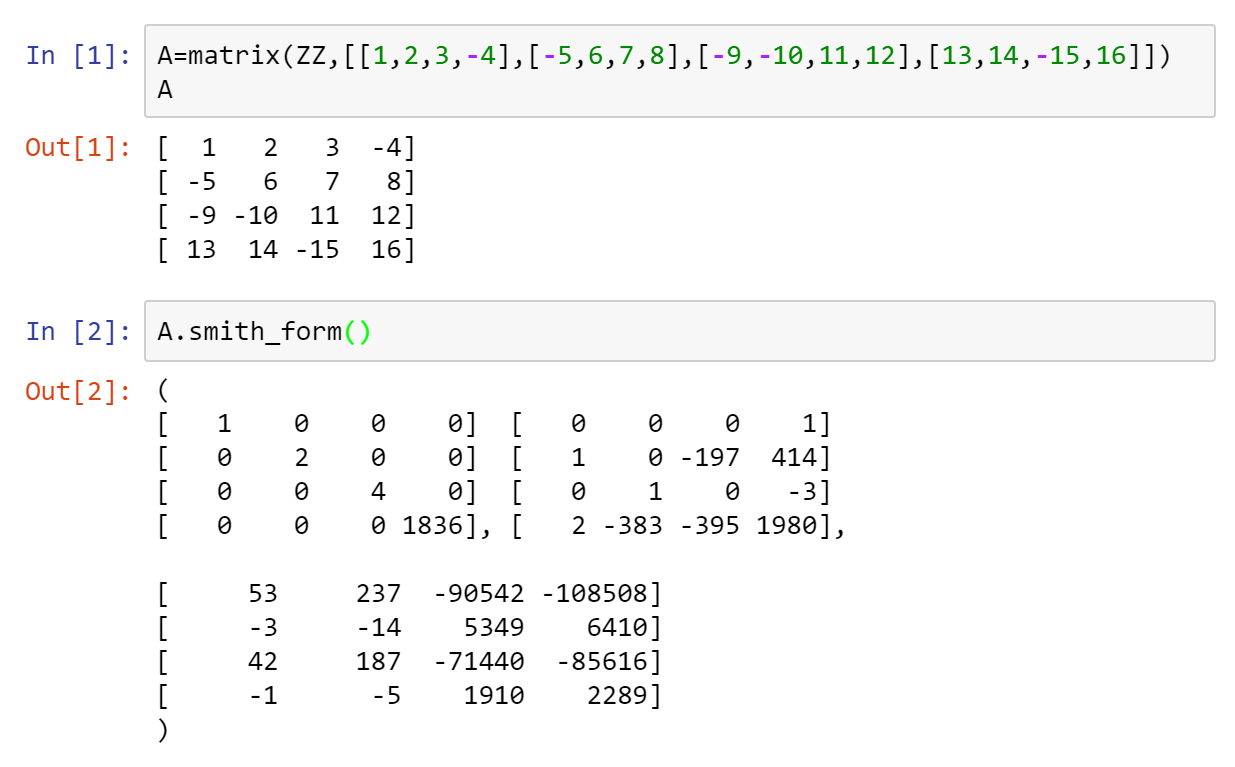
\includegraphics[scale=0.6]{smithForm}
\end{frame}

% % %
\begin{frame}[c]
The Smith normal form of the given matrix, call it $A$, is 
\[
D:=\begin{pmatrix}
1 & 0 & 0 & 0 \\
0 & 2 & 0 & 0 \\
0 & 0 & 4 & 0 \\
0 & 0 & 0 & 1836
\end{pmatrix}.
\]
The other two matrices in the output are respectively $B$ and $C$ from Theorem \ref{thm:SmithNormalForm}, so that $D=BAC$.
\end{frame}

% % % % % % % % % % 
\end{document}